% 内存
% 内存.tex

\documentclass[12pt,UTF8]{ctexbook}

% 设置纸张信息。
\input{../../../Book/common/page}

% 设置字体，并解决显示难检字问题。
\xeCJKsetup{AutoFallBack=true}
% 注意：ctexbook类已默认设置SimSun为CJKrmdefault
% 以下设置用于确保字体回退和扩展字体可用
% 仅设置扩展字体以避免与默认设置冲突
\setCJKfamilyfont{hei}{SimHei}
\setCJKfamilyfont{kai}{KaiTi}

% 目录 chapter 级别加点（.）。
\usepackage{titletoc}
\titlecontents{chapter}[0pt]{\vspace{3mm}\bf\addvspace{2pt}\filright}{\contentspush{\thecontentslabel\hspace{0.8em}}}{}{\titlerule*[8pt]{.}\contentspage}

% 支持目录点击跳转
\usepackage[colorlinks,linkcolor=blue,citecolor=blue,urlcolor=blue]{hyperref}

% 设置 part 和 chapter 标题格式。
\ctexset{
	part/name= {第,卷},
	part/number={\chinese{part}},
	chapter/name={第,篇},
	chapter/number={\arabic{chapter}}
}

% 图片相关设置。
\usepackage{graphicx}
\graphicspath{{Images/}}

% 设置署名格式。
\newenvironment{shuming}{\hfill\zihao{4}}

% 注脚每页重新编号，避免编号过大。
\usepackage[perpage]{footmisc}

% 设置段落间距
\setlength{\parskip}{0.8em plus 0.2em minus 0.1em}

% 列表格式支持，列表项向右偏移。
\usepackage{enumitem}

\usepackage{tabularx}
\usepackage{float}

\title{\heiti\zihao{0} 内存}
\author{WangFei}
\date{\today}

\begin{document}

\maketitle
\tableofcontents

\frontmatter
\chapter{前言}

本书专为完全没有计算机硬件基础的学习者设计，将带你从零开始了解内存的基本概念、工作原理和实际应用。

本书将涵盖以下内容：
\begin{itemize}
    \item 内存的基本概念和历史
    \item 内存的工作原理和内部结构
    \item 不同类型内存的特点和应用场景
    \item 内存的性能指标和选型建议
    \item 内存的安装和维护方法
\end{itemize}

让我们开始这段有趣的学习之旅吧！

\mainmatter

\part{内存基础概念}

\chapter{什么是内存}

内存（Memory）是计算机中用于临时存储数据和程序的硬件设备。它就像计算机的"工作台"，CPU在处理数据时会先将数据从硬盘读取到内存中，因为内存的速度远快于硬盘。

\section{内存的作用}

内存主要负责以下任务：

\begin{itemize}[leftmargin=2em]
    \item \textbf{临时存储}：存储正在运行的程序和数据
    \item \textbf{快速访问}：提供比硬盘快得多的数据访问速度
    \item \textbf{数据交换}：作为CPU与其他设备之间的数据中转站
\end{itemize}

简单来说，内存就是计算机"正在使用"的数据的临时存放处。

\section{内存与硬盘的区别}

很多初学者会混淆内存和硬盘，它们的主要区别如下：

\begin{table}[H]
    \centering
    \begin{tabularx}{\textwidth}{|p{3cm}|X|X|}
        \hline
        \multicolumn{1}{|c|}{\textbf{特性}} & \multicolumn{1}{c|}{\textbf{内存}} & \multicolumn{1}{c|}{\textbf{硬盘}} \\
        \hline
        存储类型 & 临时存储（断电丢失） & 永久存储（断电保留） \\
        \hline
        访问速度 & 非常快（纳秒级） & 较慢（毫秒级） \\
        \hline
        容量 & 较小（几GB到几十GB） & 很大（几百GB到几TB） \\
        \hline
        价格 & 较贵 & 较便宜 \\
        \hline
        用途 & 运行中的程序和数据 & 长期保存的文件和数据 \\
        \hline
    \end{tabularx}
    \caption{内存与硬盘对比}
    \label{tab:memory_vs_hdd}
\end{table}

\section{内存的外观}

内存通常是长条形的电路板，称为内存模块（RAM Module）：

\begin{figure}[htbp]
    \centering
    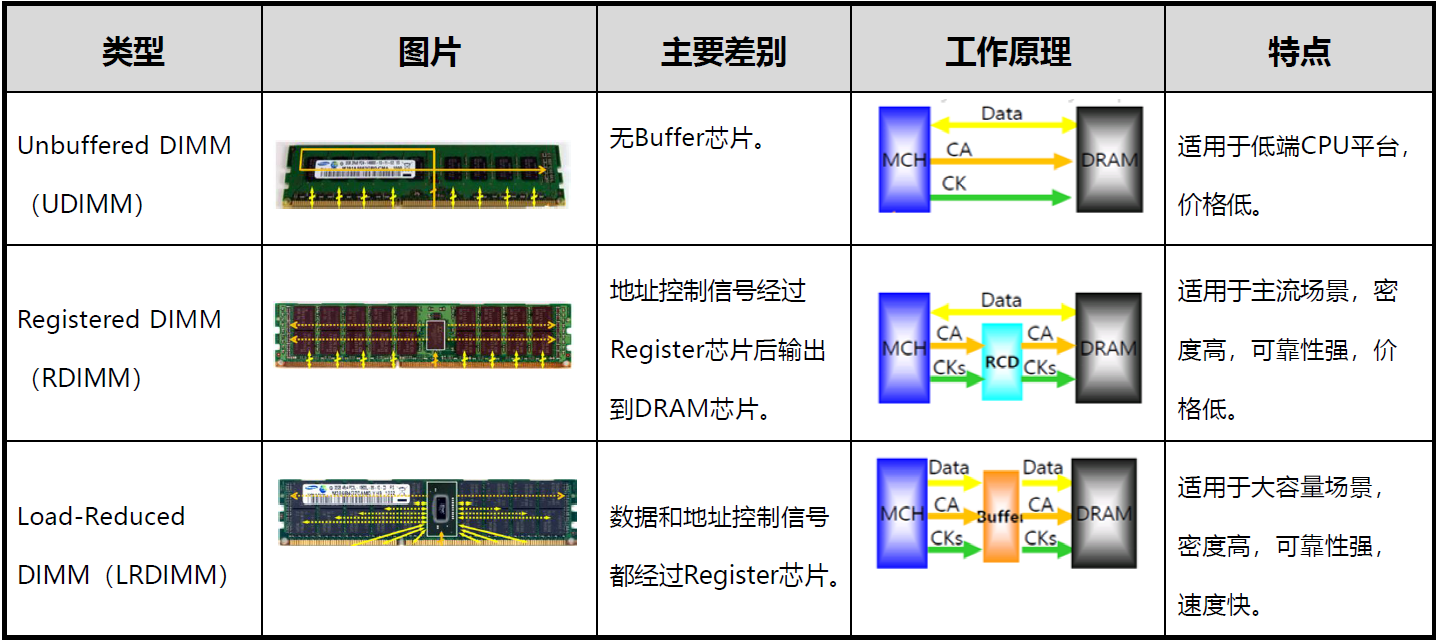
\includegraphics[width=0.6\linewidth]{memory.png}
    \caption{内存模块外观}
    \label{fig:memory外观}
\end{figure}

内存模块的特点：

\begin{enumerate}
    \item \textbf{金手指}：底部的金色触点，用于连接主板
    \item \textbf{缺口}：防止插反的防呆设计
    \item \textbf{散热片}：部分高端内存带有散热片
    \item \textbf{标签}：标注容量、频率等信息
\end{enumerate}

\chapter{内存的历史演进}

\section{早期内存}

\begin{enumerate}
    \item \textbf{磁芯内存（1950-1970年代）}：
    \begin{itemize}[leftmargin=2em]
        \item 使用小磁环存储数据
        \item 体积大、功耗高、容量小
    \end{itemize}
    
    \item \textbf{DRAM（动态随机存取内存）}：
    \begin{itemize}[leftmargin=2em]
        \item 1966年发明，使用电容存储数据
        \item 需要定期刷新，功耗较低
        \item 奠定了现代内存的基础
    \end{itemize}
\end{enumerate}

\section{现代内存时代}

\begin{enumerate}
    \item \textbf{SDRAM（同步动态RAM）}：
    \begin{itemize}[leftmargin=2em]
        \item 与CPU时钟同步
        \item 速度大幅提升
    \end{itemize}
    
    \item \textbf{DDR系列内存}：
    \begin{itemize}[leftmargin=2em]
        \item DDR：双倍数据速率
        \item DDR2、DDR3、DDR4、DDR5逐步升级
        \item 速度和带宽不断提升
    \end{itemize}
    
    \item \textbf{移动端内存}：
    \begin{itemize}[leftmargin=2em]
        \item LPDDR：低功耗DDR
        \item 用于手机、平板等移动设备
    \end{itemize}
\end{enumerate}

\chapter{内存的核心组成}

\section{内存芯片}

内存模块由多个内存芯片组成：

\begin{itemize}[leftmargin=2em]
    \item \textbf{DRAM芯片}：存储数据的核心元件
    \item \textbf{容量}：每个芯片的容量决定了整个模块的容量
    \item \textbf{封装}：常见的封装形式有TSOP、BGA等
\end{itemize}

\section{内存控制器}

内存控制器负责协调CPU与内存之间的数据传输：

\begin{enumerate}
    \item \textbf{位置}：早期在北桥芯片，现在集成在CPU内部
    \item \textbf{功能}：控制内存读写、管理内存时序
    \item \textbf{重要性}：直接影响内存性能
\end{enumerate}

\section{内存通道}

内存通道是数据传输的路径：

\begin{enumerate}
    \item \textbf{单通道}：一条数据通路
    \item \textbf{双通道}：两条并行数据通路，带宽翻倍
    \item \textbf{三通道/四通道}：更高带宽，常见于服务器
\end{enumerate}

\part{内存类型与技术}

\chapter{DDR内存家族}

\section{DDR内存发展历程}

\begin{table}[H]
    \centering
    \begin{tabular}{|p{2cm}|p{3cm}|p{3cm}|p{3cm}|p{3cm}|}
        \hline
        \textbf{类型} & \textbf{标准电压} & \textbf{峰值带宽} & \textbf{常见频率} & \textbf{引脚数} \\
        \hline
        DDR & 2.5V & 6.4 GB/s & 400 MHz & 184 \\
        \hline
        DDR2 & 1.8V & 12.8 GB/s & 800 MHz & 240 \\
        \hline
        DDR3 & 1.5V & 25.6 GB/s & 1600 MHz & 240 \\
        \hline
        DDR4 & 1.2V & 51.2 GB/s & 3200 MHz & 288 \\
        \hline
        DDR5 & 1.1V & 102.4 GB/s & 6400 MHz & 288 \\
        \hline
    \end{tabular}
    \caption{DDR内存规格对比}
    \label{tab:ddr_specs}
\end{table}

\section{DDR4与DDR5的区别}

\begin{enumerate}
    \item \textbf{带宽}：DDR5带宽是DDR4的两倍
    \item \textbf{电压}：DDR5更低（1.1V vs 1.2V）
    \item \textbf{架构}：DDR5采用双通道设计（每个模块内两个通道）
    \item \textbf{PMIC}：DDR5集成电源管理芯片
\end{enumerate}

\chapter{其他类型内存}

\section{SRAM（静态随机存取内存）}

\begin{enumerate}
    \item \textbf{特点}：速度快、不需要刷新
    \item \textbf{缺点}：成本高、容量小
    \item \textbf{应用}：CPU缓存（L1/L2/L3）
\end{enumerate}

\section{SDRAM与DDR的区别}

\begin{table}[H]
    \centering
    \begin{tabularx}{\textwidth}{|p{4cm}|X|X|}
        \hline
        \multicolumn{1}{|c|}{\textbf{对比项}} & \multicolumn{1}{c|}{\textbf{SDRAM}} & \multicolumn{1}{c|}{\textbf{DDR}} \\
        \hline
        数据传输 & 单倍数据速率 & 双倍数据速率 \\
        \hline
        时钟效率 & 每时钟周期传输1次 & 每时钟周期传输2次 \\
        \hline
        速度 & 较慢 & 较快 \\
        \hline
        电压 & 3.3V & 2.5V及以下 \\
        \hline
    \end{tabularx}
    \caption{SDRAM与DDR对比}
    \label{tab:sdram_vs_ddr}
\end{table}

\section{LPDDR（低功耗DDR）}

\begin{enumerate}
    \item \textbf{特点}：低功耗、小体积
    \item \textbf{应用}：手机、平板、笔记本电脑
    \item \textbf{版本}：LPDDR3、LPDDR4、LPDDR5
\end{enumerate}

\part{内存性能与选型}

\chapter{内存性能指标}

\section{容量}

\begin{enumerate}
    \item \textbf{定义}：内存可以存储的数据量
    \item \textbf{单位}：GB（千兆字节）
    \item \textbf{常见容量}：4GB、8GB、16GB、32GB、64GB
    \item \textbf{选择建议}：
    \begin{itemize}[leftmargin=2em]
        \item 日常办公：8GB够用
        \item 游戏娱乐：16GB起步
        \item 专业创作：32GB及以上
    \end{itemize}
\end{enumerate}

\section{频率}

\begin{enumerate}
    \item \textbf{定义}：内存工作的时钟频率
    \item \textbf{单位}：MHz（兆赫兹）
    \item \textbf{常见频率}：
    \begin{itemize}[leftmargin=2em]
        \item DDR4：2400MHz、2666MHz、3200MHz、3600MHz
        \item DDR5：4800MHz、5600MHz、6400MHz
    \end{itemize}
    \item \textbf{注意}：频率需要CPU和主板支持
\end{enumerate}

\section{时序}

\begin{enumerate}
    \item \textbf{定义}：内存读写操作的延迟时间
    \item \textbf{表示}：如CL16-18-18-36
    \item \textbf{含义}：
    \begin{itemize}[leftmargin=2em]
        \item CL：列地址选通延迟
        \item tRCD：行地址到列地址延迟
        \item tRP：行预充电时间
        \item tRAS：行激活时间
    \end{itemize}
    \item \textbf{选择}：时序越小，性能越好
\end{enumerate}

\section{带宽}

\begin{enumerate}
    \item \textbf{定义}：内存每秒可传输的数据量
    \item \textbf{计算公式}：带宽 = 频率 × 位宽 × 通道数 / 8
    \item \textbf{单位}：GB/s（千兆字节/秒）
\end{enumerate}

\chapter{内存选购指南}

\section{兼容性检查}

\begin{enumerate}
    \item \textbf{内存类型}：确认主板支持DDR4还是DDR5
    \item \textbf{插槽数量}：了解主板有几个内存插槽
    \item \textbf{最大容量}：确认主板支持的最大内存容量
    \item \textbf{频率支持}：确认CPU和主板支持的内存频率
\end{enumerate}

\section{品牌推荐}

\begin{enumerate}
    \item \textbf{金士顿（Kingston）}：老牌厂商，品质可靠
    \item \textbf{威刚（ADATA）}：性价比高，产品线丰富
    \item \textbf{海力士（Hynix）}：内存颗粒大厂，质量优秀
    \item \textbf{三星（Samsung）}：技术领先，性能出色
    \item \textbf{芝奇（G.SKILL）}：高端超频内存专家
\end{enumerate}

\section{内存型号识别}

\begin{figure}[htbp]
    \centering
    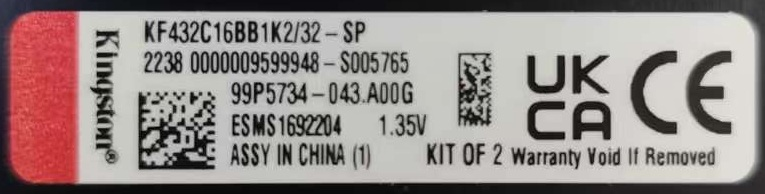
\includegraphics[width=0.7\linewidth]{Kingston.jpg}
    \caption{金士顿内存型号识别}
    \label{fig:kingston_model}
\end{figure}

\begin{figure}[htbp]
    \centering
    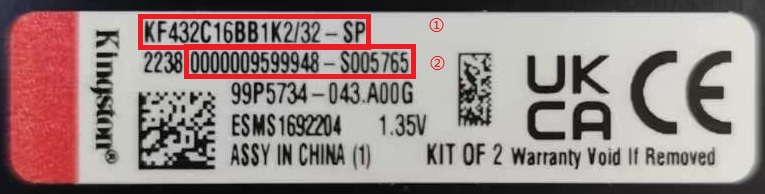
\includegraphics[width=0.7\linewidth]{Kingston-1.jpg}
    \caption{金士顿内存编号细节}
    \label{fig:kingston_detail}
\end{figure}

\begin{figure}[htbp]
    \centering
    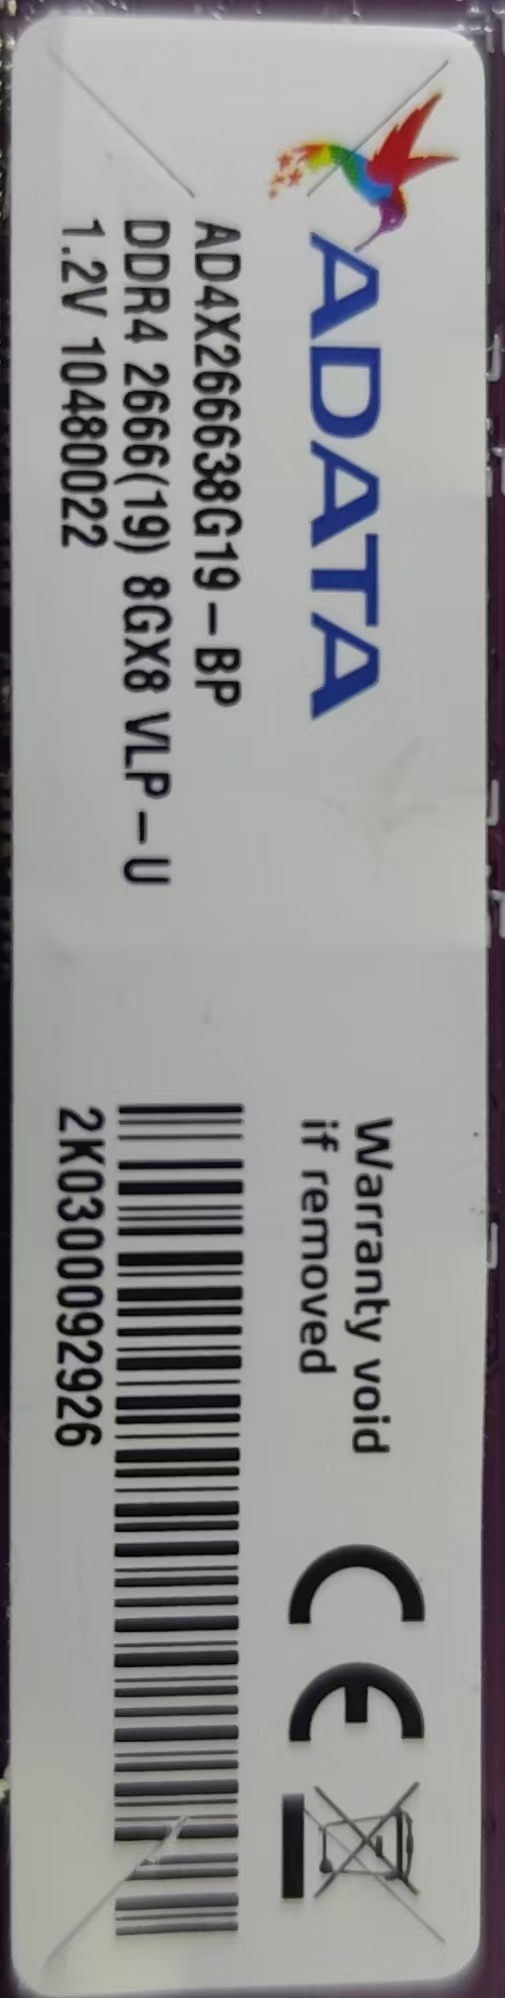
\includegraphics[width=0.7\linewidth]{ADATA.jpg}
    \caption{威刚内存型号识别}
    \label{fig:adata_model}
\end{figure}

\begin{figure}[htbp]
    \centering
    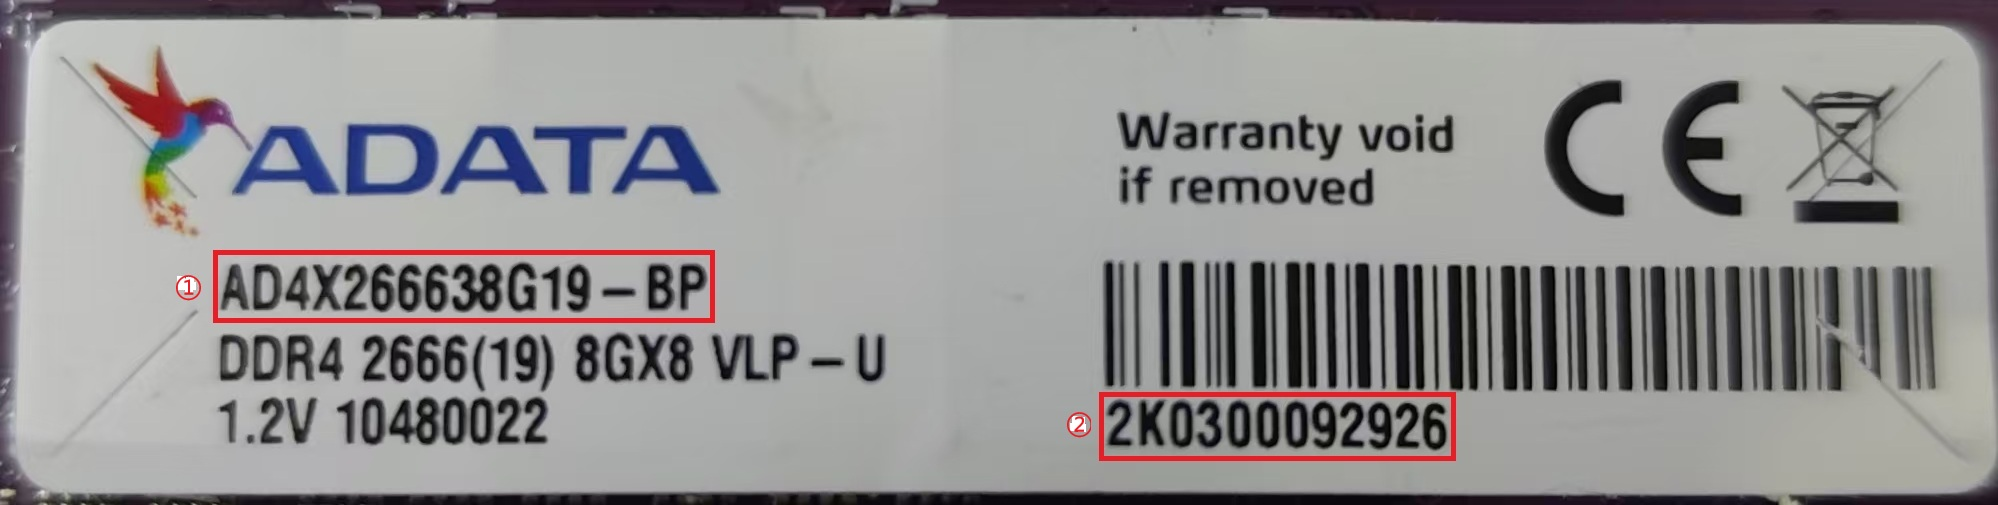
\includegraphics[width=0.7\linewidth]{ADATA-1.jpg}
    \caption{威刚内存编号细节}
    \label{fig:adata_detail}
\end{figure}

\begin{figure}[htbp]
    \centering
    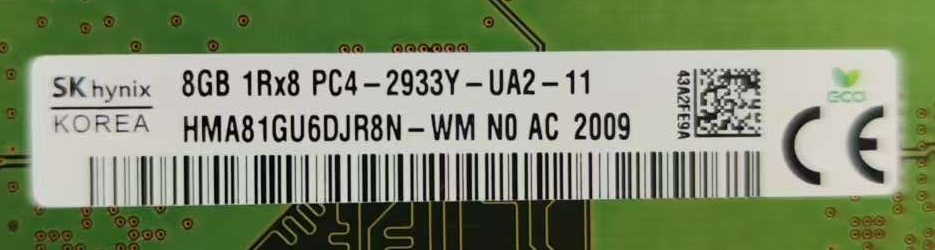
\includegraphics[width=0.7\linewidth]{hynix.png}
    \caption{海力士内存型号识别}
    \label{fig:hynix_model}
\end{figure}

\begin{figure}[htbp]
    \centering
    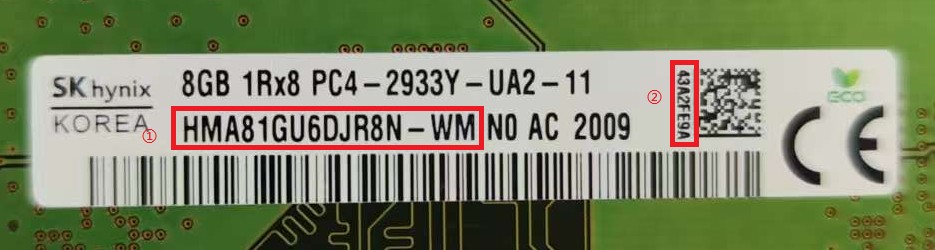
\includegraphics[width=0.7\linewidth]{hynix-1.png}
    \caption{海力士内存编号细节}
    \label{fig:hynix_detail}
\end{figure}

\part{实践与维护}

\chapter{内存安装}

\section{安装步骤}

\begin{enumerate}
    \item \textbf{准备工作}：
    \begin{itemize}[leftmargin=2em]
        \item 关闭电脑电源
        \item 拔掉电源线
        \item 释放静电（触摸金属物体）
    \end{itemize}
    
    \item \textbf{找到内存插槽}：
    \begin{itemize}[leftmargin=2em]
        \item 主板上长条形的插槽
        \item 通常有2-4个插槽
    \end{itemize}
    
    \item \textbf{安装内存}：
    \begin{itemize}[leftmargin=2em]
        \item 对准缺口位置
        \item 均匀用力按下两端
        \item 听到"咔嗒"声表示安装到位
    \end{itemize}
    
    \item \textbf{双通道配置}：
    \begin{itemize}[leftmargin=2em]
        \item 通常插在相同颜色的插槽
        \item 参考主板说明书
    \end{itemize}
\end{enumerate}

\section{注意事项}

\begin{itemize}[leftmargin=2em]
    \item 不要用力过猛，以免损坏插槽
    \item 确保内存完全插入
    \item 安装前确认内存类型与主板兼容
\end{itemize}

\chapter{内存维护与故障排查}

\section{常见问题}

\begin{enumerate}
    \item \textbf{电脑无法开机}：
    \begin{itemize}[leftmargin=2em]
        \item 检查内存是否插好
        \item 尝试重新插拔内存
        \item 检查内存是否与主板兼容
    \end{itemize}
    
    \item \textbf{系统不稳定、蓝屏}：
    \begin{itemize}[leftmargin=2em]
        \item 可能是内存不兼容或损坏
        \item 运行内存测试工具（如MemTest86）
        \item 尝试单条内存测试
    \end{itemize}
    
    \item \textbf{内存容量显示不正确}：
    \begin{itemize}[leftmargin=2em]
        \item 检查是否所有内存都被识别
        \item 确认主板支持的最大容量
    \end{itemize}
\end{enumerate}

\section{内存测试}

\begin{enumerate}
    \item \textbf{MemTest86}：专业内存测试工具
    \item \textbf{Windows内存诊断}：系统自带工具
    \item \textbf{测试建议}：测试时间不少于1小时
\end{enumerate}

\chapter{内存发展趋势}

\section{当前发展方向}

\begin{enumerate}
    \item \textbf{DDR5普及}：更高带宽、更低功耗
    \item \textbf{大容量内存}：单条32GB、64GB成为主流
    \item \textbf{集成内存}：部分CPU集成内存（如苹果M系列）
\end{enumerate}

\section{未来展望}

\begin{enumerate}
    \item \textbf{DDR6}：预计带宽翻倍
    \item \textbf{3D堆叠内存}：更高密度
    \item \textbf{新内存技术}：如MRAM、RRAM等非易失性内存
\end{enumerate}

\part{附录}

\chapter{内存常见问题解答}

\section{常见问题}

\begin{enumerate}
    \item \textbf{Q: 内存越大越好吗？}
    \\A: 不一定，够用即可。超过实际需求的内存不会带来性能提升。
    
    \item \textbf{Q: 不同品牌的内存可以混用吗？}
    \\A: 可以，但建议使用相同规格（容量、频率、时序）的内存，以保证兼容性和性能。
    
    \item \textbf{Q: 内存需要升级吗？}
    \\A: 如果经常出现内存不足的提示，或者运行大型软件时卡顿，可以考虑升级。
    
    \item \textbf{Q: 笔记本电脑内存可以更换吗？}
    \\A: 部分笔记本可以更换，部分是板载内存无法更换，需要查看电脑规格。
\end{enumerate}

\chapter{参考资料}

\begin{itemize}[leftmargin=2em]
    \item JEDEC官方网站：https://www.jedec.org
    \item 金士顿官方网站：https://www.kingston.com
    \item 威刚官方网站：https://www.adata.com
    \item 海力士官方网站：https://www.skhynix.com
\end{itemize}

\backmatter

\end{document}